% !TeX spellcheck = it_IT
\newpage
\section{Logica proposizionale}
\subsection{Sintassi}
La sintassi è la seguente, rappresentata in BNF:
\begin{equation}
	\begin{split}
		formula & \to formulaAtomica \vert formulaComplessa \\
		formulaAtomica & \to True \vert False \vert simbolo \\
		simbolo & \to P \vert Q \vert R \vert \ldots \\
		formulaComplessa & \to \neg formula \\
		&\vert (formula \land formula) \\
		& \vert (formula \lor formula)\\
		& \vert (formula \Rightarrow formula)\\
		& \vert (formula \Leftrightarrow formula)
	\end{split}
\end{equation}

\subsection{Semantica}
La logica proposizionale segue una semantica \textbf{composizionale}, dove il significato di una frase è determinato dal significato dei suoi componenti a partire dai \textit{simboli proposizionali}. Di seguito la ravola di verità:
\begin{table}[h!]
	\centering
	\begin{tabular}{|cc|ccccc|}
		\hline
		$P$ & $Q$ & $\neg P$ & $P \land Q$ & $P \lor Q$ & $ P \Rightarrow Q$ & $P \Leftrightarrow Q$\\
		\hline
		false & false & true & false & false & true & true \\
		false & true & true & false & true & true & false \\
		true & false & false & false & true & false & false \\
		true & true & false & true & true & true & true\\
		\hline
	\end{tabular}
\end{table}

\subsection{Conseguenza logica}
\begin{definition}[Conseguenza logica]
	Una formula $\alpha$ è una conseguenza logica di un insieme di formule KB se e solo se in ogni modello di KB, anche $\alpha$ è vera ($KB \models \alpha$).
\end{definition}
Indichiamo con $M(KB)$ i modelli dell'insieme di formule in KB e con $M(\alpha)$ l'insieme delle interpretazioni che rendono $\alpha$ vera, ovvero i suoi \textbf{modelli}.
\begin{equation}
	KB \models \alpha \Leftrightarrow M(KB) \subseteq M(\alpha)
\end{equation}

\subsubsection{Model checking}
Un modo per determinare la conseguenza logica è quello di enumere i \textit{modelli} e mostrare che la formula $\alpha$ vale in tutti quelli in cui è vera la KB.

\begin{example}[Wumpus World]
	\label{example:wumpus_world_model_checking}
	Partendo dall'esempio \ref{example:wumpus_world} abbiamo che la KB iniziale, $KB_0$, è costituita dalle regole descritte nella definizione dell'esercizio:
	\begin{gather*}
		\neg W_{1,1} \quad \neg P_{1,1} \\
		B_{2,1} \Leftrightarrow (P_{1,1} \lor P_{2,2,} \lor P_{3,1})\\
		B_{1,1} \Leftrightarrow (P_{1,2} \lor P_{2,1})\\
		\vdots
	\end{gather*}
	Il primo passo dell'agente è spostarsi in $[2,1]$ dato che in $[1,1]$ non ha percepito niente. Abbiamno quindi:
	\begin{equation*}
		KB_1 = KB_0 \cup \{\neg B_{1,1}, B_{2,1}, \neg F_{1,1}, \neg F_{2,1}, \ldots\}
	\end{equation*}
	e rappresentiamo le domande sulla presenza o meno di pozzi come:
	\begin{equation*}
		\begin{split}
			KB_1 \models \neg P_{1,2} \\
			KB_1 \models \neg P_{2,2} \\
			KB_1 \models \neg P_{3,1} \\
		\end{split}
	\end{equation*}
	Sapendo da $KB_0$ che non ci sono pozzi nella casella $[1,1]$ e che c'è un pozzo nella stanza adiacente solo se ci percepisce la brezza, formuliamo le seguenti proposizioni:
	\begin{equation*}
		\begin{split}
			& B_{1,1} \Leftrightarrow (P_{1,2} \lor P_{2,1}) \\
			& B_{2,1} \Leftrightarrow (P_{1,1} \lor P_{2,2} \lor P_{3,1})
		\end{split}
	\end{equation*}
	e concludiamo che non c'è brezza in $[1,1]$ e c'è in $[2,1]$, ovvero $\neg B_{1,1}$ e $B_{2,1}$.\\
	Ci rimangono quindi tre configurazioni possibili dato che abbiamo:
	\begin{gather*}
		KB_1 \models \neg P_{1,2}\\
		KB_1 \models P_{2,2}\lor P_{3,1}
	\end{gather*}
	e sono quelle in cui i pozzi sono in $[3,1]$ oppure in $[2,2]$ oppure in entrambi.i
\end{example}

\subsubsection{SAT}
Un altro approccio alla dimostrazione della conseguenza logica si basa su tre principi:
\begin{itemize}
	\item \textbf{Equivalenza logica}: due formule $\alpha$ e $\beta$sono equivalenti se sono vere nello stesso insieme di modelli
	\begin{equation}
		\alpha \equiv \beta \Leftrightarrow \alpha \models \beta\land\beta\models\alpha
	\end{equation}
	Alcune leggi fondamentali per l'equivalenza sono:
	\begin{itemize}
		\item \textit{Commutatività}: $(\alpha\land\beta)\equiv(\beta\land\alpha)\quad(\alpha\lor\beta)\equiv(\beta\lor\alpha)$
		\item \textit{Associatività}: $((\alpha\land\beta)\land\gamma)\equiv(\alpha\land(\beta\land\gamma))\quad((\alpha\lor\beta)\lor\gamma)\equiv(\alpha\lor(\beta\lor\gamma))$
		\item \textit{Eliminazione della doppia negazione}: $\neg(\neg\alpha)$
		\item \textit{Contrapposizione}: $(\alpha\Rightarrow\beta)\equiv(\neg\beta\Rightarrow\neg\alpha)$
		\item \textit{Eliminazione dell'implicazione}: $(\alpha\Rightarrow\beta)\equiv(\neg\alpha\lor\beta)$
		\item \textit{Eliminazione del bicondizionale}: $(\alpha\Leftrightarrow\beta)\equiv((\alpha\Rightarrow\beta)\land(\beta\Rightarrow\alpha))$
		\item \textit{De Morgan}: $\neg(\alpha \land\beta)\equiv(\neg\alpha\lor\neg\beta)\quad\neg(\alpha \lor\beta)\equiv(\neg\alpha\land\neg\beta)$
		\item \textit{Distributività}: $(\alpha\land(\beta\lor\gamma))\equiv((\alpha\land\beta)\lor(\alpha\land\gamma)\quad(\alpha\lor(\beta\land\gamma))\equiv((\alpha\lor\beta)\land(\alpha\lor\gamma))$
	\end{itemize}
	\item \textbf{Validità}: una formula $\alpha$ è valida se e solo se è vera in tutte le sue interpretazioni. In quel caso sono anche dette \textbf{tatutologie}.
	\begin{theorem}[Teorema di deduzione e refutazione]
		Date due formule $\alpha$ e $\beta$, allora $\alpha \models\beta \Leftrightarrow (\alpha\Rightarrow\beta)$. Possiamo riscriverlo, usando le leggi appena elencate, anche come $\alpha\models\beta \Leftrightarrow (\alpha \land \neg\beta)$, che ci permette di fare la dimostrazione per \textbf{assurdo}.
	\end{theorem}
	\item \textbf{Soddisfacibilità}: una formula $\alpha$ è soddisfacibile se e solo se esiste una interpretazione in cui $\alpha$ è vera (ovvero se esiste un modello di $\alpha$). La determinazione della soddisfacibilità è il problema \textbf{SAT}.
\end{itemize}
Si noti che \textit{validità} e \textit{soddisfacibilità} sono connesse:
\begin{itemize}
	\item $\alpha$ è valida se e solo se $\neg\alpha$ è insoddisfacibile
	\item $\alpha$ è soddisfacibvile se e solo se $\neg\alpha$ non è valida
\end{itemize}
\begin{definition}[Forma a clausole]
	La forma a clausole è la \textbf{forma normale congiuntiva} (CNF), ovvero una congiunzione di disgiunzioni di letterali (un simbolo o la sua negazione). È sempre possibile ottenerla con trasformazioni che preservano l'equivalenza logica.
\end{definition}
Per eseguire una trasformazione in forma a clausole bisogna seguire i seguenti passi:
\begin{enumerate}
	\item Eliminazione del $\Leftrightarrow$
	\item Eliminazione del $\Rightarrow$
	\item Portare le negazioni all'interno tramite De Morgan
	\item Distribuire $\lor$ su $\land$
\end{enumerate}

\begin{example}
	Partendo dall'esempio \ref{example:wumpus_world}, trasformiamo $B_{1,1} \Leftrightarrow (P_{1,2}\lor P_{2,1})$:
	\begin{enumerate}
		\item $(B_{1,1} \Rightarrow (P_{1,2} \lor P_{2,1})) \land ((P_{1,2} \lor P_{2,1}) \Rightarrow B_{1,1})$
		\item $(\neg B_{1,1} \lor (P_{1,2} \lor P_{2,1})) \land (\neg(P_{1,2} \lor P_{2,1}) \lor B_{1,1})$
		\item $(\neg B_{1,1} \lor (P_{1,2} \lor P_{2,1})) \land ((\neg P_{1,2} \land \neg P_{2,1}) \lor B_{1,1})$
		\item $(\neg B_{1,1} \lor P_{1,2} \lor P_{2,1}) \land (\neg(P_{1,2} \lor B_{1,1}) \land (\neg P_{2,1} \lor B_{1,1})$
	\end{enumerate}
	che possiamo riscrivere come
	\begin{equation*}
		\{\neg B_{1,1}, P_{1,2}, P_{2,1}\}\{\neg P_{1,2}, B_{1,1,}\}\{\neg P_{2,1}, B_{1,1}\}
	\end{equation*}
\end{example}

\subsubsection{Deduzione}
Un altro modo per dimostrare la conseguenza logica è utilizzare un \textbf{sistema di deduzione}, che denotiamo come $KB \vdash A$. La deduzione avviene specificando delle \textbf{regole di inferenza} con le seguenti caratteristiche:
\begin{itemize}
	\item Devono derivare \textbf{solo} formule che sono conseguenza logica
	\item Devono derivare \textbf{tutte} le formule che sono conseguenza logica
\end{itemize}
\begin{definition}[Correttezza]
	Tutto ciò che è derivabile è conseguenza logica, le regole preservano la verità.
	\begin{equation}
		KB \vdash \alpha \Rightarrow KB \models \alpha
	\end{equation}
\end{definition}
\begin{definition}[Completezza]
	Tutto ciò che è conseguenza logica è ottenibile tramite il sistema di deduzione.
	\begin{equation}
		KB \models \alpha \Rightarrow KB \vdash \alpha
	\end{equation}
\end{definition}
Alcune regole di inferenza sono:
\begin{gather}
	\frac{\alpha \Rightarrow \beta, \quad \alpha}{\beta} \quad\quad\text{Modu ponens}\\
	\frac{\alpha \land \beta}{\alpha} \quad\quad\text{Eliminazione dell\'AND}\\
	\frac{\alpha \Leftrightarrow \beta}{(\alpha \Rightarrow \beta) \land (\beta \Rightarrow \alpha)} \quad\quad\text{Introduzione della doppia implicazione}\\
	\frac{(\alpha \Rightarrow \beta) \land (\beta \Rightarrow \alpha)}{\alpha \Leftrightarrow \beta} \quad\quad\text{Eliminazione della doppia implicazione}
\end{gather}

\begin{example}[Wumpus]
	Partendo dalle stesse assunzioni fatte nell'esempio \ref{example:wumpus_world_model_checking}, voglio chiedermi se posso dimostrare con le regole di inferenza che non c'è un pozzo in $[1,1]$, ovvero $\neg P_{1,2}$.
	\begin{align*}
		R_6: (B_{1,1} \Rightarrow (P_{1,2} \lor P_{2,1})) \land ((P_{1,2} \lor P_{2,1}) \Rightarrow B_{1,1}) && (R_2, \Leftrightarrow E) \\
		R_7: (P_{1,2} \lor P_{2,1}) \Rightarrow B_{1,1} && (R_6,\land E)\\
		R_8: \neg B_{1,1} \Rightarrow \neg (P_{1,2} \lor P_{2,1}) && (R_7, \text{contrapposizione}) \\
		R_9: \neg(P_{1,2} \lor P_{2,1}) && (R_4, R_8, \text{Modus ponens}) \\
		R_{10}: \neg P_{1,2} \land \neg P_{2,1} && (R_9, \text{De Morgan})\\
		R_{11}: \neg P_{1,2} && (R_10, \land E)
	\end{align*}
\end{example}
\noindent Anche la deduzione può quindi essere visto come problema di ricerca, dove vanno definite:
\begin{itemize}
	\item \textbf{Direzione} della ricerca: nella dimostrazione di teoremi conviene procedere all'\textit{indietro}
	\item \textbf{Strategia} della ricerca:
	\begin{itemize}
		\item \textit{Completezza}: le regole della deduzione naturale sono un un insieme completo, se lo è anche l'algoritmo siamo a posto
		\item \textit{Efficienza}: è un problema decidibile ma NP-Completo
	\end{itemize}
\end{itemize}
In generale per risolvere una proposizione meno regole abbiamo e meglio è, senza però rinunciare alla completezza.\\
Dati $l$ e $m$ letterali positivi o negativi e $l_i$ e $m_j$ di segno opposto, la regola di risoluzione possiamo scriverla in generale come:
\begin{equation}
	\frac{\{l_1, \ldots, l_i, \ldots, l_k\}\{m_1, \ldots, m_j, \ldots, m_n\}}{\{l_1, \ldots, l_{i-1}, l_{i+1}, \ldots, l_k\}\{m_1, \ldots, m_{j-1}, m_{j+1}, \ldots, m_n\}}
\end{equation}
da cui poi possiamo costruirci un \textbf{grafo di risoluzione}.

\newpage
\subsection{Algoritmi}
Di seguito alcuni algoritmi per determinare se è vera una conseguenza logica a partire da una KB.
\subsubsection{TV-Consegue}
Questo algoritmo enumera tutte le possibili interpretazioni di KB, e per ciascuna interpretazione se soddisfa la KB controlla che soddisfi anche $\alpha$. Basta trovare una singola interpretazione che soddisfa la KB ma non $\alpha$ per determinare una risposta negativa. Avremo quindi, dati $k$ simboli, $2^k$ possibili interpretazioni.
\label{alg:tv_consegue}
\begin{lstlisting}
	function TV-Consegue?(KB, a) // Restituisce true oppure false
	inputs: KB, la base di conoscenza, una formula della logica proposizionale
	a, la query, una formula della logica proposizionale
	simboli = una lista dei simboli proposizionali contenuti in KB e a
	return TV-Verifica-Tutto(KB, a, simboli, { })
	
	function TV-Verifica-Tutto(KB, a, simboli, modello) // Restituisce true oppure false
	if Vuoto?(simboli) then
	if PL-Vero?(KB, modello) then return PL-Vero?(a, modello)
	else return true // Quando KB false, restituisce sempre true
	else do
	P = Primo(simboli); resto = Resto(simboli)
	return TV-Verifica-Tutto(KB, a, resto, modello = {P = true})
	and
	TV-Verifica-Tutto(KB, a, resto, modello = {P = false})
\end{lstlisting}

\begin{example}
	Supponiamo di voler verificare la seguente conseguenza logica:
	\begin{equation*}
		(\neg a\lor b)\land(a \lor c) \models (b \lor c)
	\end{equation*}
	Ci costruiamo la tabella di verità:
	\begin{table}[!h]
		\centering
		\begin{tabular}{|ccc|cc|}
			\hline
			$a$&$b$&$c$&$\neg a \lor b$ & $a \lor c$ \\
			\hline
			T & T & T & T & T\\
			T & T& F & T & T \\
			T & F &T&F&T\\
			T&F&F&F&T\\
			F&T&T&T&T\\
			F&T&F&T&F\\
			F&F&T&T&T\\
			F&F&F&T&F\\
			\hline
		\end{tabular}
	\end{table}
	Per poi selezionare solo le righe in cui la KB è vera e verificare se la nostra formula è sempre vera:
	\begin{table}[!h]
		\centering
		\begin{tabular}{|ccc|cc|c|}
			\hline
			$a$&$b$&$c$&$\neg a \lor b$ & $a \lor c$ & $b\lor c$\\
			\hline
			T & T & T & T & T & T\\
			T & T& F & T & T & T\\
			F&T&T&T&T & T\\
			F&F&T&T&T&T\\
			\hline
		\end{tabular}
	\end{table}
	Quindi la risposta è sì.\\
	Applicando l'algoritmo \ref{alg:tv_consegue} abbiamo la seguente esecuzione:
	\begin{lstlisting}
		TV-VERIFICA-TUTTO(KB, formula, [a, b, c], { })
		TV-VERIFICA-TUTTO(KB, formula, [b, c], {a=T})
		TV-VERIFICA-TUTTO(KB, formula, [c], {a=T, b=T})
		TV-VERIFICA-TUTTO(KB, formula, [ ], {a=T, b=T, c=T}) // OK
		TV-VERIFICA-TUTTO(KB, formula, [ ], {a=T, b=T, c=F}) // OK
		TV-VERIFICA-TUTTO(KB, formula, [c], {a=T, b=F})
		TV-VERIFICA-TUTTO(KB, formula, [ ], {a=T, b=F, c=T}) // OK
		TV-VERIFICA-TUTTO(KB, formula, [ ], {a=T, b=F, c=F}) // OK
		TV-VERIFICA-TUTTO(KB, formula, [b, c], [a=F])
		etc...
	\end{lstlisting}
\end{example}
\subsubsection{DPLL}
\label{alg:dpll}
Questo algoritmo parte da una KB in forma a clausole e prende in input una formula in CNF ed enumera ricorsivamente in profondità tutte le possibili interpretazioni alla ricerca di un modello. Per avere un miglioramento sull'algoritmo \ref{alg:tv_consegue} applico tre clausole:
\begin{itemize}
	\item \textbf{Terminazione anticipata}: si può decidere sulla verità di una clausola anche con interpretazioni parziali, ovvero quando ho degli \textit{OR} basta che un simbolo sia vero mentre quando ho degli \textit{AND} basta che unpo sia falso per rendere falsa l'intera interpretazione
	\item \textbf{Euristica dei simboli puri}: un simbolo puro è un simbolo che appare con lo stesso segno in tutte le clausole (trascurando eventualmente quelle già rese vere). Possono poi essere assegnati a True se il letterale è positivo o a False se è negativo
	\item \textbf{Euristica delle clausole unitarie}: una clausola in cui è rimasto un solo letterale non assegnato
\end{itemize}

\begin{lstlisting}
	function DPLL-Soddisfacibile?(s) returns true oppure false
	inputs: s, una formula della logica proposizionale
	clausole = insieme di clausole nella rappresentazione CNF di s
	simboli = una lista di tutti i simboli proposizionali in s
	return DPLL(clausole, simboli, { })
	
	function DPLL(clausole, simboli, modello) returns true oppure false
	if ogni clausola in clausole vera in modello then return true
	if qualche clausola in clausole falsa in modello then return false
	P, valore = Trova-Simbolo-Puro(simboli, clausole, modello)
	if P diverso da null then return DPLL(clausole, simboli - P, modello = {P = valore})
	P, valore = Trova-Clausola-Unitaria(clausole, modello)
	if P diverso da null then return DPLL(clausole, simboli-P, modello = {P = valore})
	P = Primo(simboli); resto = Resto(simboli)
	return	DPLL(clausole, resto, modello = {P = true})
	or
	DPLL(clausole, resto, modello = {P = false})
\end{lstlisting}

\begin{example}
	Supponiamo di voler verificare la seguente conseguenza logica:
	\begin{equation*}
		\{\neg B_{1,1}, P_{1,2}, P_{2,1}\}\{\neg P_{1,2}, B_{1,1}\}\{\neg P_{2,1}, B_{1,1}\}\{\neg B_{1,1}\} \models \{\neg P_{1,2}\}
	\end{equation*}
	Aggiungiamo alla KB la clausola $\{P_{1,2}\}$ e verifichiamo con SAT se l'insieme è insoddisfacibile:
	\begin{enumerate}
		\item La clausola $\{P_{1,2}\}$ è unitaria, quindi $P_{1,2}=True$. Di conseguenza $\{\neg B_{1,1}, P_{1,2}, P_{2,1}\}$ e $\{P_{1,2}\}$ sono soddisfatte e rimaniamo con
		\begin{equation*}
			\{\neg P_{1,2}, B_{1,1}\}\{\neg P_{2,1}, B_{1,1}\}\{\neg B_{1,1}\}
		\end{equation*}
		\item $P_{2,1}$ è un simbolo puro ed essendo negativo sarà uguale a False, quindi la clausola $\{\neg P_{2,1}, B_{1,1}\}$ è soddisfatta e rimaniamo con
		\begin{equation*}
			\{\neg P_{1,2}, B_{1,1}\}\{\neg B_{1,1}\}
		\end{equation*}
	\end{enumerate}
	Dato che non esistono modelli possiamo dire che $\neg P_{1,2}$ è conseguenza logica della KB
\end{example}
\noindent Questo algoritmo è \textbf{completo} e \textbf{termina sempre}. Alcuni miglioramenti sono:
\begin{itemize}
	\item Se possibile scomporre in sotto problemi indipendenti (quando non hanno simboli in comune)
	\item Ordinare le variabili per frequenza di comparizione
	\item Backtracing intelligente
\end{itemize}

\subsubsection{WalkSAT}
\label{alg:walksat}
Definiamo la formulazione di un problema SAT in ambito locale:
\begin{itemize}
	\item \textbf{Stati}: sono le interpretazioni, assegnamenti completi
	\item \textbf{Obiettivo}: un assegnamento che soddisfa tutte le clausole (\textit{modello})
\end{itemize}
Si parte da un assegnamento \textit{casuale} e ad ogni passo si cambia il valore di un simbolo proposizionale (\textbf{flip}). La valutazione di uno stato avviene controllando il numero di clausole soddisfatte.

Ad ogni passo viene scelta a caso una clausola non soddisfatta e individua un simbolo da modificare, scegliendo con probabilità $p$ tra:
\begin{itemize}
	\item \textbf{Random walk}: il simbolo è scelto a caso
	\item \textbf{Ottimizzazione}: viene scelto il simbolo che rende più clausole soddisfatte
\end{itemize}
Dopo un certo numero di flip predefinito, l'algoritmo si arrende.
\begin{lstlisting}
	function WalkSAT(clausole, p, max_flips) returns un modello o fallimento
	modello = assegnamento casuale di valori di verita ai simboli in clausole
	
	for i = 1 to max_flips do
	if modello soddisfa clausole then return modello
	clausola = una clausola, falsa in modello, scelta casualmente nell'insieme clausole
	if Random(0, 1) =< p then inverti il valore in modello di un simbolo scelto
	casualmente in clausola
	else inverti il valore di verita del simbolo in clausole che massimizza il numero
	di clausole soddisfatte
	
	return fallimento
\end{lstlisting}

\begin{example}[WalkSAT]
	L'obiettivo è quello di massimizzare il numero di clausole soddisfatte tra le seguenti:
	\begin{equation*}
		\{\neg B_{1,1}, P_{1,2}, P_{2,1}\}\{\neg P_{1,2}, B_{1,1}\}\{\neg P_{2,1}, B_{1,1}\}\{\neg B_{1,1}\}
	\end{equation*}
	Un esempio di esecuzione dell'algoritmo è il seguente:
	\begin{enumerate}
		\item Configurazione di \textit{partenza}: $[B_{1,1}=F,P_{1,2}=T,P_{2,1}=T]$
		\item \textit{Random walk}: la prima e la quarta clausola sono soddisfatte, scelgo seconda e faccio un flip a caso di $B_{1,1}$ ottenendo $[B_{1,1}=T,P_{1,2}=T,P_{2,1}=T]$
		\item L'unica non soddisfatta è la quarta, posso solo fare un flip di $B_{1,1}$ ottenendo $[B_{1,1}=F,P_{1,2}=T,P_{2,1}=T]$
		\item \textit{Random walk}: la prima e la quarta clausola sono soddisfatte, scelgo la seconda e faccio un flip a caso di $P_{1,2}$ ottenendo $[B_{1,1}=F,P_{1,2}=F,P_{2,1}=T]$
		\item \textit{Ottimizzazione}: l'unica non soddisfatta è la terza, faccio un flip di $P_{2,1}$ ottenendo $[B_{1,1}=F,P_{1,2}=F,P_{2,1}=F]$
	\end{enumerate}
\end{example}

Se il limite $max_flips = \infty$ e l'insieme di clausole è soddisfacibile, prima o poi termina, ma  se non lo è non terminerà mai. Non possiamo quindi usarlo per verificare l'insoddisfacibilità.

\subsubsection{Confronto}
Se un problema è \textbf{sotto-vincolato} (ha molte soluzioni) è più probabile che \textit{WalkSAT} trovi una soluzione in tempi brevi.
\begin{example}[3-SAT]
	Dato il seguente problema 3-SAT, ovvero con clausole di 3 letterali:
	\begin{equation*}
		\{\neg D, \neg B, C\} \{B, \neg A, \neg C\} \{\neg C, \neg B, E\} \{E, \neg D, B\} \{B, E, \neg C\}
	\end{equation*}
	Abbiamo $32$ possibili interpretazioni con $16$ possibili soluzioni. Questo sarebbe facile da risolvere con \textit{Walk-SAT}.
\end{example}
\noindent È importante nel capire il livello di difficoltà di un problema SAT il rapporto tra numero di \textbf{clausole} e numero di \textbf{simboli}
\begin{equation}
	\frac{m}{n}
\end{equation}
Infatti, più è grande il rapporto e più vincolato è il problema.
\begin{example}
	Supponiamo di avere $n=50$ simboli e di avere $m$ clausole che variano.
	\begin{center}
		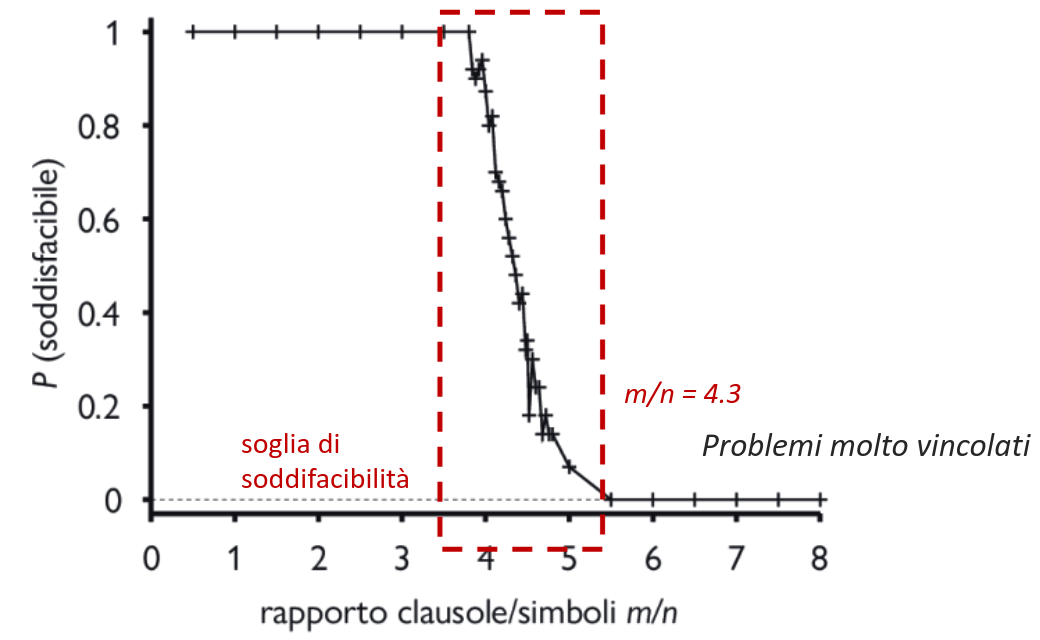
\includegraphics[scale=0.2]{prob_sodd.png}
	\end{center}
	Su 100 problemi generati a caso vediamo che $4.3$ è la soglia oltre la quale un problema diventa difficile da risolvere.
\end{example}
\noindent Vediamo il \textbf{confronto} tra l'algoritmo \hyperref[alg:dpll]{DPLL} e \hyperref[alg:walksat]{WalkSAT}:
\begin{center}
	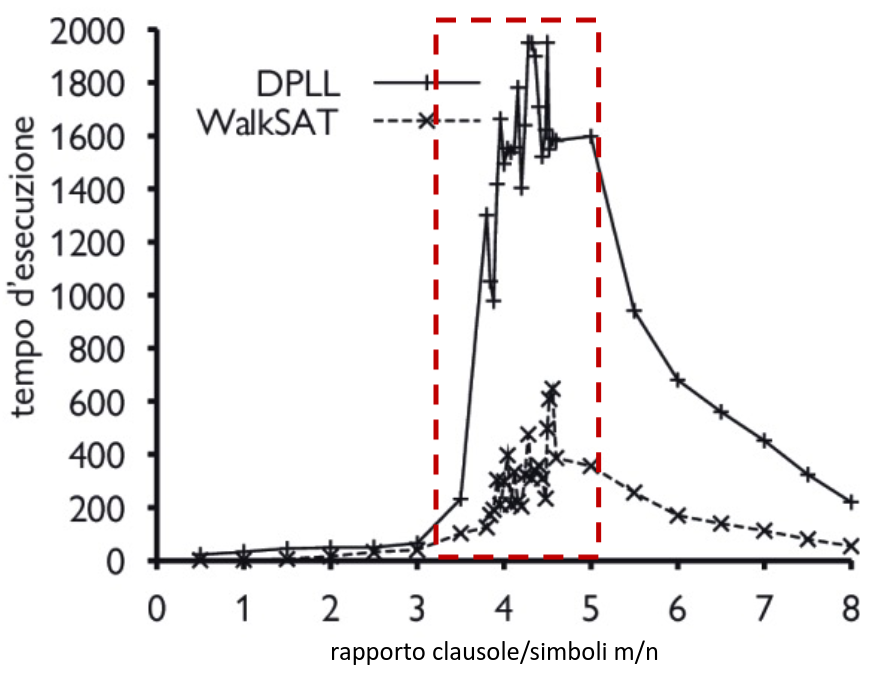
\includegraphics[scale=0.3]{dpll_vs_walksat.png}
\end{center}
Notiamo che i problemi vicini alla \textit{soglia di soddisfacibilità} sono molto più difficili da risolvere rispetto a quelli più lontani. Inoltre vediamo che quando un problema è poco vincolato i due algoritmi performano allo stesso modo mentre intorno alla soglia \textit{WalkSAT} è nettamente migliore.